\documentclass[a4paper, 11pt]{article}
\usepackage{amsmath}
\usepackage{graphicx}
\usepackage{geometry}
\usepackage{listings}
\geometry{scale=0.8}
\linespread{1.5}
\usepackage{hyperref}
\usepackage{listings}


\title{	
\normalfont \normalsize
\textsc{School of Data and Computer Science, Sun Yat-sen University} \\ [25pt] %textsc small capital letters
\rule{\textwidth}{0.5pt} \\[0.4cm] % Thin top horizontal rule
\huge  E10 Naive Bayes (C++/Python)\\ % The assignment title
\rule{\textwidth}{2pt} \\[0.5cm] % Thick bottom horizontal rule
\author{16110917 Zhaoshuai Liu}
\date{\normalsize\today}
}

\begin{document}
\maketitle
\tableofcontents
\newpage

\section{Datasets}
\label{sec:datasets}

The UCI dataset (\url{http://archive.ics.uci.edu/ml/index.php}) is the most widely used dataset for machine learning. If you are interested in other datasets in other areas, you can refer to \url{https://www.zhihu.com/question/63383992/answer/222718972}.

Today's experiment is conducted with the \textbf{Adult Data Set} which can be found in \url{http://archive.ics.uci.edu/ml/datasets/Adult}.
\begin{figure}[ht]
\centering
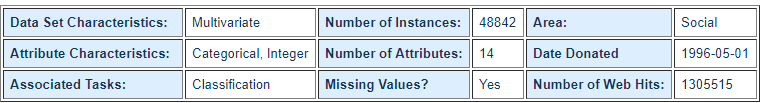
\includegraphics[width=17cm]{dataset}
\end{figure}

You can also find 3 related files in the current folder, \texttt{adult.name} is the description of \textbf{Adult Data Set}, \texttt{adult.data} is the training set, and \texttt{adult.test} is the testing set. There are 14 attributes in this dataset:
\begin{lstlisting}{language=Python}
>50K, <=50K.

1. age: continuous.
2. workclass: Private, Self-emp-not-inc, Self-emp-inc, Federal-gov, Local-gov,
State-gov, Without-pay, Never-worked.
3. fnlwgt: continuous.
4. education: Bachelors, Some-college, 11th, HS-grad, Prof-school, Assoc-acdm,
Assoc-voc, 9th, 7th-8th, 12th, Masters, 5. 1st-4th, 10th, Doctorate, 5th-6th,
Preschool.
5. education-num: continuous.
6. marital-status: Married-civ-spouse, Divorced, Never-married, Separated,
Widowed, Married-spouse-absent, Married-AF-spouse.
7. occupation: Tech-support, Craft-repair, Other-service, Sales,
Exec-managerial, Prof-specialty, Handlers-cleaners, Machine-op-inspct,
Adm-clerical,Farming-fishing,Transport-moving,Priv-house-serv,Protective-serv,
Armed-Forces.
8. relationship: Wife,Own-child,Husband,Not-in-family,Other-relative,Unmarried.
9. race: White, Asian-Pac-Islander, Amer-Indian-Eskimo, Other, Black.
10. sex: Female, Male.
11. capital-gain: continuous.
12. capital-loss: continuous.
13. hours-per-week: continuous.
14. native-country: United-States, Cambodia,England,Puerto-Rico,Canada,Germany,
Outlying-US(Guam-USVI-etc),India,Japan,Greece, South,China,Cuba,Iran,Honduras,
Philippines, Italy, Poland, Jamaica, Vietnam, Mexico, Portugal, Ireland, France,
Dominican-Republic,Laos,Ecuador,Taiwan, Haiti, Columbia,Hungary,Guatemala,
Nicaragua,Scotland,Thailand,Yugoslavia,El-Salvador, Trinadad&Tobago,Peru,Hong,
Holand-Netherlands.

\end{lstlisting}
\textbf{Prediction task is to determine whether a person makes over 50K a year.}

\section{Naive Bayes}

Naive Bayes is a simple technique for constructing classifiers: models that assign class labels to problem instances, represented as vectors of feature values, where the class labels are drawn from some finite set. It is not a single algorithm for training such classifiers, but a family of algorithms based on a common principle: all naive Bayes classifiers assume that \textbf{the value of a particular feature is independent of the value of any other feature}, given the class variable.

For example, a fruit may be considered to be an apple if it is red, round, and about 10 cm in diameter. A naive Bayes classifier considers each of these features to contribute independently to the probability that this fruit is an apple, regardless of any possible correlations between the color, roundness, and diameter features.

Naive Bayes methods are a set of supervised learning algorithms based on applying Bayes’ theorem with the ``naive'' assumption of conditional independence between every pair of features given the value of the class variable. Bayes’ theorem states the following relationship, given class variable $y$ and dependent feature vector $x_1$ through $x_n$:
$$P(y\ |\ x_1,...,x_n)=\frac{P(y)P(x_1,...,x_n\ |\ y)}{P(x_1,...,x_n)}$$
Using the naive conditional independence assumption that
$$P(x_i\ |\ y,x_1,...,x_{i-1},x_{x+1},...,x_n)=P(x_i\ |\ y)$$,
for all $i$, this relationship is simplified to
$$P(y\ | x_1,...,x_n)=\frac{P(y)\prod_{i=1}^n P(x_i\ |\ y)}{P(x_1,...,x_n)}$$
Since $P(x_1,...,x_n)$ is constant given the input, we can use the following classification rule:
$$P(y\ | x_1,...,x_n)\propto P(y)\prod_{i=1}^n P(x_i\ |\ y)$$
$$\hat{y}=\arg\max\limits_y P(y)\prod^n_{i=1}P(x_i\ |\ y),$$
and we can use Maximum A Posteriori (MAP) estimation to estimate $P(y)$ and $P(x_i\ |\ y)$, the former is then the relative frequency of class $y$ in the training set.

The different naive Bayes classifiers differ mainly by the assumptions they make regarding the distribution of $P(x_i\ |\ y)$.

\begin{itemize}
	\item When attribute values are discrete, $P(x_i\ |\ y)$ can be easily computed according to the training set.
	\item When attribute values are continuous, an assumption is made that the values associated with each class are distributed according to Gaussian i.e., Normal Distribution. For example, suppose the training data contains a continuous attribute $x$. We first segment the data by the class, and then compute the mean and variance of $x$ in each class. Let $\mu_k$ be the mean of the values in $x$ associated with class $y_k$, and let $\sigma_k^2$ be the variance of the values in $x$ associated with class $y_k$. Suppose we have collected some observation value $x_i$. Then, the probability distribution of $x_i$ given a class $y_k$, $P(x_i\ | y_k)$ can be computed by plugging $x_i$ into the equation for a Normal distribution parameterized by $\mu_k$ and $\sigma_k^2$. That is,
	$$P(x=x_i\ |\ y=y_k)=\frac{1}{\sqrt{2\pi\sigma_k^2}}e^{-\frac{(x_i-\mu_k)^2}{2\sigma_k^2}}$$

\end{itemize}

\section{Task}
\begin{itemize}
\item Given the training dataset \texttt{adult.data} and the testing dataset \texttt{adult.test}, please accomplish the prediction task to determine whether a person makes over 50K a year in \texttt{adult.test} by using Naive Bayes algorithm (C++ or Python), and compute the accuracy.
\item Note: keep an eye on the discrete and continuous attributes.
\item Please finish the experimental report named \texttt{E10\_YourNumber.pdf}, and send it to \texttt{ai\_2018@foxmail.com}
\end{itemize}

\section{Codes}
\begin{lstlisting}[language=Python,frame=single]
import numpy as np
import math
import scipy.stats as st

train_data = open("adult.data")
moreThan50K = 0
lessThan50K = 0
P_moreThan50K = 0
P_lessThan50K = 0
tol_count = 0

age_more = []
workclass_more = {'Private': 0, 'Self-emp-not-inc': 0, 'Self-emp-inc': 0,
             'Federal-gov': 0, 'Local-gov': 0, 'State-gov': 0,
             'Without-pay': 0, 'Never-worked': 0}
fnlwgt_more = []
education_more = {'Bachelors': 0, 'Some-college': 0, '11th': 0,
             'HS-grad': 0, 'Prof-school': 0, 'Assoc-acdm': 0,
             'Assoc-voc': 0, '9th': 0, '7th-8th': 0, '12th': 0,
             'Masters': 0, '5': 0, '1st-4th': 0, '10th': 0,
             'Doctorate': 0, '5th-6th': 0, 'Preschool': 0}
education_num_more = []
marital_status_more = {'Married-civ-spouse': 0, 'Divorced': 0,
                  'Never-married': 0, 'Separated': 0, 'Widowed': 0,
                  'Married-spouse-absent': 0, 'Married-AF-spouse': 0}
occupation_more = {'Tech-support': 0, 'Craft-repair': 0,
              'Other-service': 0, 'Sales': 0, 'Exec-managerial': 0,
              'Prof-specialty': 0, 'Handlers-cleaners': 0,
              'Machine-op-inspct': 0, 'Adm-clerical': 0,
              'Farming-fishing': 0, 'Transport-moving': 0,
              'Priv-house-serv': 0, 'Protective-serv': 0,
              'Armed-Forces': 0}

realationship_more = {'Wife': 0, 'Own-child': 0, 'Husband': 0,
                'Not-in-family': 0, 'Other-relative': 0,
                'Unmarried': 0}

race_more = {'White': 0, 'Asian-Pac-Islander': 0,
        'Amer-Indian-Eskimo': 0, 'Other': 0,
        'Black': 0}

sex_more = {'Female': 0, 'Male': 0}

capital_gain_more = []
capital_loss_more = []
hours_per_week_more = []

native_country_more = {'United-States': 0, 'Cambodia': 0,
                  'England': 0, 'Puerto-Rico': 0, 'Canada': 0,
                  'Germany': 0, 'Outlying-US(Guam-USVI-etc)': 0,
                  'India': 0, 'Japan': 0, 'Greece': 0, 'South': 0,
                  'China': 0, 'Cuba': 0, 'Iran': 0, 'Honduras': 0,
                  'Philippines': 0, 'Italy': 0, 'Poland': 0,
                  'Jamaica': 0, 'Vietnam': 0, 'Mexico': 0,
                  'Portugal': 0, 'Ireland': 0, 'France': 0,
                  'Dominican-Republic': 0, 'Laos': 0, 'Ecuador': 0,
                  'Taiwan': 0, 'Haiti': 0, 'Columbia': 0, 'Hungary': 0,
                  'Guatemala': 0, 'Nicaragua': 0, 'Scotland': 0,
                  'Thailand': 0, 'Yugoslavia': 0, 'El-Salvador': 0,
                  'Trinadad&Tobago': 0, 'Peru': 0, 'Hong': 0,
                  'Holand-Netherlands': 0}
age_less = []
workclass_less = {'Private': 0, 'Self-emp-not-inc': 0,
                'Self-emp-inc': 0, 'Federal-gov': 0,
                'Local-gov': 0, 'State-gov': 0,
                'Without-pay': 0, 'Never-worked': 0}
fnlwgt_less = []
education_less = {'Bachelors': 0, 'Some-college': 0,
                  '11th': 0, 'HS-grad': 0,
                  'Prof-school': 0, 'Assoc-acdm': 0,
                  'Assoc-voc': 0, '9th': 0,
                  '7th-8th': 0, '12th': 0, 'Masters': 0,
                  '5': 0, '1st-4th': 0,
                  '10th': 0, 'Doctorate': 0,
                  '5th-6th': 0, 'Preschool': 0}
education_num_less = []
marital_status_less = {'Married-civ-spouse': 0, 'Divorced': 0,
                       'Never-married': 0, 'Separated': 0,
                       'Widowed': 0, 'Married-spouse-absent': 0,
                       'Married-AF-spouse': 0}
occupation_less = {'Tech-support': 0, 'Craft-repair': 0,
                   'Other-service': 0, 'Sales': 0,
                   'Exec-managerial': 0, 'Prof-specialty': 0,
                   'Handlers-cleaners': 0, 'Machine-op-inspct': 0,
                   'Adm-clerical': 0, 'Farming-fishing': 0,
                   'Transport-moving': 0, 'Priv-house-serv': 0,
                   'Protective-serv': 0, 'Armed-Forces': 0}

realationship_less = {'Wife': 0, 'Own-child': 0, 'Husband': 0,
                      'Not-in-family': 0, 'Other-relative': 0,
                      'Unmarried': 0}

race_less = {'White': 0, 'Asian-Pac-Islander': 0,
             'Amer-Indian-Eskimo': 0, 'Other': 0,
             'Black': 0}
sex_less = {'Female': 0, 'Male': 0}
capital_gain_less = []
capital_loss_less = []
hours_per_week_less = []
native_country_less = {'United-States': 0, 'Cambodia': 0,
                       'England': 0, 'Puerto-Rico': 0,
                       'Canada': 0, 'Germany': 0,
                       'Outlying-US(Guam-USVI-etc)': 0,
                       'India': 0, 'Japan': 0, 'Greece': 0,
                       'South': 0, 'China': 0, 'Cuba': 0, 'Iran': 0,
                       'Honduras': 0, 'Philippines': 0, 'Italy': 0,
                       'Poland': 0, 'Jamaica': 0,
                       'Vietnam': 0, 'Mexico': 0, 'Portugal': 0,
                       'Ireland': 0, 'France': 0,
                       'Dominican-Republic': 0, 'Laos': 0,
                       'Ecuador': 0, 'Taiwan': 0, 'Haiti': 0,
                       'Columbia': 0, 'Hungary': 0, 'Guatemala': 0,
                       'Nicaragua': 0, 'Scotland': 0,
                       'Thailand': 0, 'Yugoslavia': 0,
                       'El-Salvador': 0, 'Trinadad&Tobago': 0,
                       'Peru': 0, 'Hong': 0, 'Holand-Netherlands': 0}

while 1:
    line = train_data.readline()
    line = line[:-1]
    if not line:
        break
    line = line.split(', ')
    if '?' in line:
        continue
    tol_count += 1
    if line[-1] == '>50K':
        moreThan50K += 1
        age_more.append(int(line[0]))
        workclass_more[line[1]] += 1
        fnlwgt_more.append(int(line[2]))
        education_more[line[3]] += 1
        education_num_more.append(int(line[4]))
        marital_status_more[line[5]] += 1
        occupation_more[line[6]] += 1
        realationship_more[line[7]] += 1
        race_more[line[8]] += 1
        sex_more[line[9]] += 1
        capital_gain_more.append(int(line[10]))
        capital_loss_more.append(int(line[11]))
        hours_per_week_more.append(int(line[12]))
        native_country_more[line[13]] += 1
    elif line[-1] == '<=50K':
        lessThan50K += 1
        age_less.append(int(line[0]))
        workclass_less[line[1]] += 1
        fnlwgt_less.append(int(line[2]))
        education_less[line[3]] += 1
        education_num_less.append(int(line[4]))
        marital_status_less[line[5]] += 1
        occupation_less[line[6]] += 1
        realationship_less[line[7]] += 1
        race_less[line[8]] += 1
        sex_less[line[9]] += 1
        capital_gain_less.append(int(line[10]))
        capital_loss_less.append(int(line[11]))
        hours_per_week_less.append(int(line[12]))
        native_country_less[line[13]] += 1
train_data.close()

P_moreThan50K = moreThan50K / tol_count
P_lessThan50K = lessThan50K / tol_count

avg_age_more = np.mean(age_more)
std_age_more = np. var(age_more)
std_age_more = math.pow(std_age_more, 0.5)

avg_age_less = np.mean(age_less)
std_age_less = np. var(age_less)
std_age_less = math.pow(std_age_less, 0.5)

avg_fnlwgt_more = np.mean(fnlwgt_more)
std_fnlwgt_more = np. var(fnlwgt_more)
std_fnlwgt_more = math.pow(std_fnlwgt_more, 0.5)

avg_fnlwgt_less = np.mean(fnlwgt_less)
std_fnlwgt_less = np. var(fnlwgt_less)
std_fnlwgt_less = math.pow(std_fnlwgt_less, 0.5)

avg_education_num_more = np.mean(education_num_more)
std_education_num_more = np. var(education_num_more)
std_education_num_more = math.pow(std_education_num_more, 0.5)

avg_education_num_less = np.mean(education_num_less)
std_education_num_less = np. var(education_num_less)
std_education_num_less = math.pow(std_education_num_less, 0.5)

avg_capital_gain_more = np.mean(capital_gain_more)
std_capital_gain_more = np. var(capital_gain_more)
std_capital_gain_more = math.pow(std_capital_gain_more, 0.5)

avg_capital_gain_less = np.mean(capital_gain_less)
std_capital_gain_less = np. var(capital_gain_less)
std_capital_gain_less = math.pow(std_capital_gain_less, 0.5)

avg_capital_loss_more = np.mean(capital_loss_more)
std_capital_loss_more = np. var(capital_loss_more)
std_capital_loss_more = math.pow(std_capital_loss_more, 0.5)

avg_capital_loss_less = np.mean(capital_loss_less)
std_capital_loss_less = np. var(capital_loss_less)
std_capital_loss_less = math.pow(std_capital_loss_less, 0.5)

avg_hours_per_week_more = np.mean(hours_per_week_more)
std_hours_per_week_more = np. var(hours_per_week_more)
std_hours_per_week_more = math.pow(std_hours_per_week_more, 0.5)

avg_hours_per_week_less = np.mean(hours_per_week_less)
std_hours_per_week_less = np. var(hours_per_week_less)
std_hours_per_week_less = math.pow(std_hours_per_week_less, 0.5)

tol_test = 0
true_test = 0
num = 0
test_data = open('adult.test')
while 1:
    line_ = test_data.readline()
    line_ = line_[:-1]
    if not line_:
        break
    num += 1
    line_ = line_.split(', ')
    if '?' in line_ or num == 1:
        continue
    tol_test += 1
    age = int(line_[0])
    workclass = line_[1]
    fnlwgt = int(line_[2])
    education = line_[3]
    education_num = int(line_[4])
    marital_status = line_[5]
    occupation = line_[6]
    realationship = line_[7]
    race = line_[8]
    sex = line_[9]
    capital_gain = int(line_[10])
    capital_loss = int(line_[11])
    hours_per_week = int(line_[12])
    native_country = line_[13]
    truth = line_[14]

    P_over = st.norm.pdf(age, avg_age_more, std_age_more) * \
             (workclass_more[workclass]/moreThan50K) * \
             st.norm.pdf(fnlwgt, avg_fnlwgt_more, std_fnlwgt_more) * \
             (education_more[education]/moreThan50K) * \
             st.norm.pdf(education_num, \
             avg_education_num_more, std_education_num_more) * \
             (marital_status_more[marital_status]/moreThan50K) * \
             (occupation_more[occupation]/moreThan50K) * \
             realationship_more[realationship]/moreThan50K * \
             race_more[race]/moreThan50K * \
             sex_more[sex]/moreThan50K * \
             st.norm.pdf(capital_gain, avg_capital_gain_more, \
             std_capital_gain_more) * st.norm.pdf(
             capital_loss, avg_capital_loss_more, \
             std_capital_loss_more) * st.norm.pdf(
             hours_per_week, avg_hours_per_week_more, \
             std_hours_per_week_more) * \
             native_country_more[native_country]/moreThan50K * \
             P_moreThan50K

    P_under = st.norm.pdf(age, avg_age_less, std_age_less) * \
              (workclass_less[workclass]/lessThan50K) * \
              st.norm.pdf(fnlwgt, avg_fnlwgt_less, \
              std_fnlwgt_less) * \
              (education_less[education]/lessThan50K) * \
              st.norm.pdf(education_num, avg_education_num_less, \
              std_education_num_less) * \
              (marital_status_less[marital_status]/lessThan50K) * \
              (occupation_less[occupation]/lessThan50K) * \
              realationship_less[realationship]/lessThan50K * \
              race_less[race]/lessThan50K * \
              sex_less[sex]/lessThan50K * \
              st.norm.pdf(capital_gain, avg_capital_gain_less, \
              std_capital_gain_less) * st.norm.pdf(
              capital_loss, avg_capital_loss_less, \
              std_capital_loss_less) * st.norm.pdf(
              hours_per_week, avg_hours_per_week_less, \
              std_hours_per_week_less) * \
              native_country_less[native_country]/lessThan50K * \
              P_lessThan50K

    result = 0
    if P_over > P_under:
        result = '>50K.'
    else:
        result = '<=50K.'
    if result == truth:
        true_test += 1
test_data.close()
print("The number of correct predictions is:")
print(true_test)
print("The number of all predictions is:")
print(tol_test)
print("The accuracy of predictions is:")
print(true_test/tol_test)


\end{lstlisting}
\section{Results}
\begin{figure}[h]
  \centering

  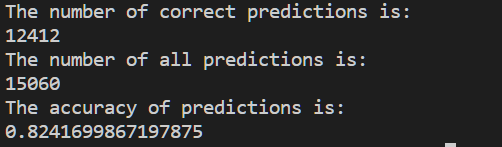
\includegraphics[width=14cm]{result.png}
\end{figure}
%\clearpage
%\bibliography{E:/Papers/LiuLab}
%\bibliographystyle{apalike}
\end{document}
%%% Local Variables:
%%% mode: latex
%%% TeX-master: t
%%% End:
